\chapter{Einleitung}
\label{kap:einleitung}

\section{Aufgabenstellung}

Mobile Bauzaunfelder werden auf Baustellen und in Mietparks liegend gestapelt;
für Inventur und Abrechnung muss die Anzahl der Felder eines Stapels bekannt
sein. Bei 50 bis 200 Feldern pro Stapel ist die Handzählung langsam und
fehleranfällig. Die Aufnahme erfolgt frontal auf die Stirnseite des Stapels,
sodass pro Feld das Ende seiner Rahmenrohre sichtbar ist: ein Kreisring aus
hellem, verzinktem Material mit dunkler Bohrung
(Abbildung~\ref{abb:realstapel}). Die Zählaufgabe wird damit zu einer
Detektionsaufgabe -- \enquote{counting by detection} --, bei der die Zahl der
detektierten Stirnflächen die Zahl der Felder bestimmt.

\begin{figure}[htbp]
  \centering
  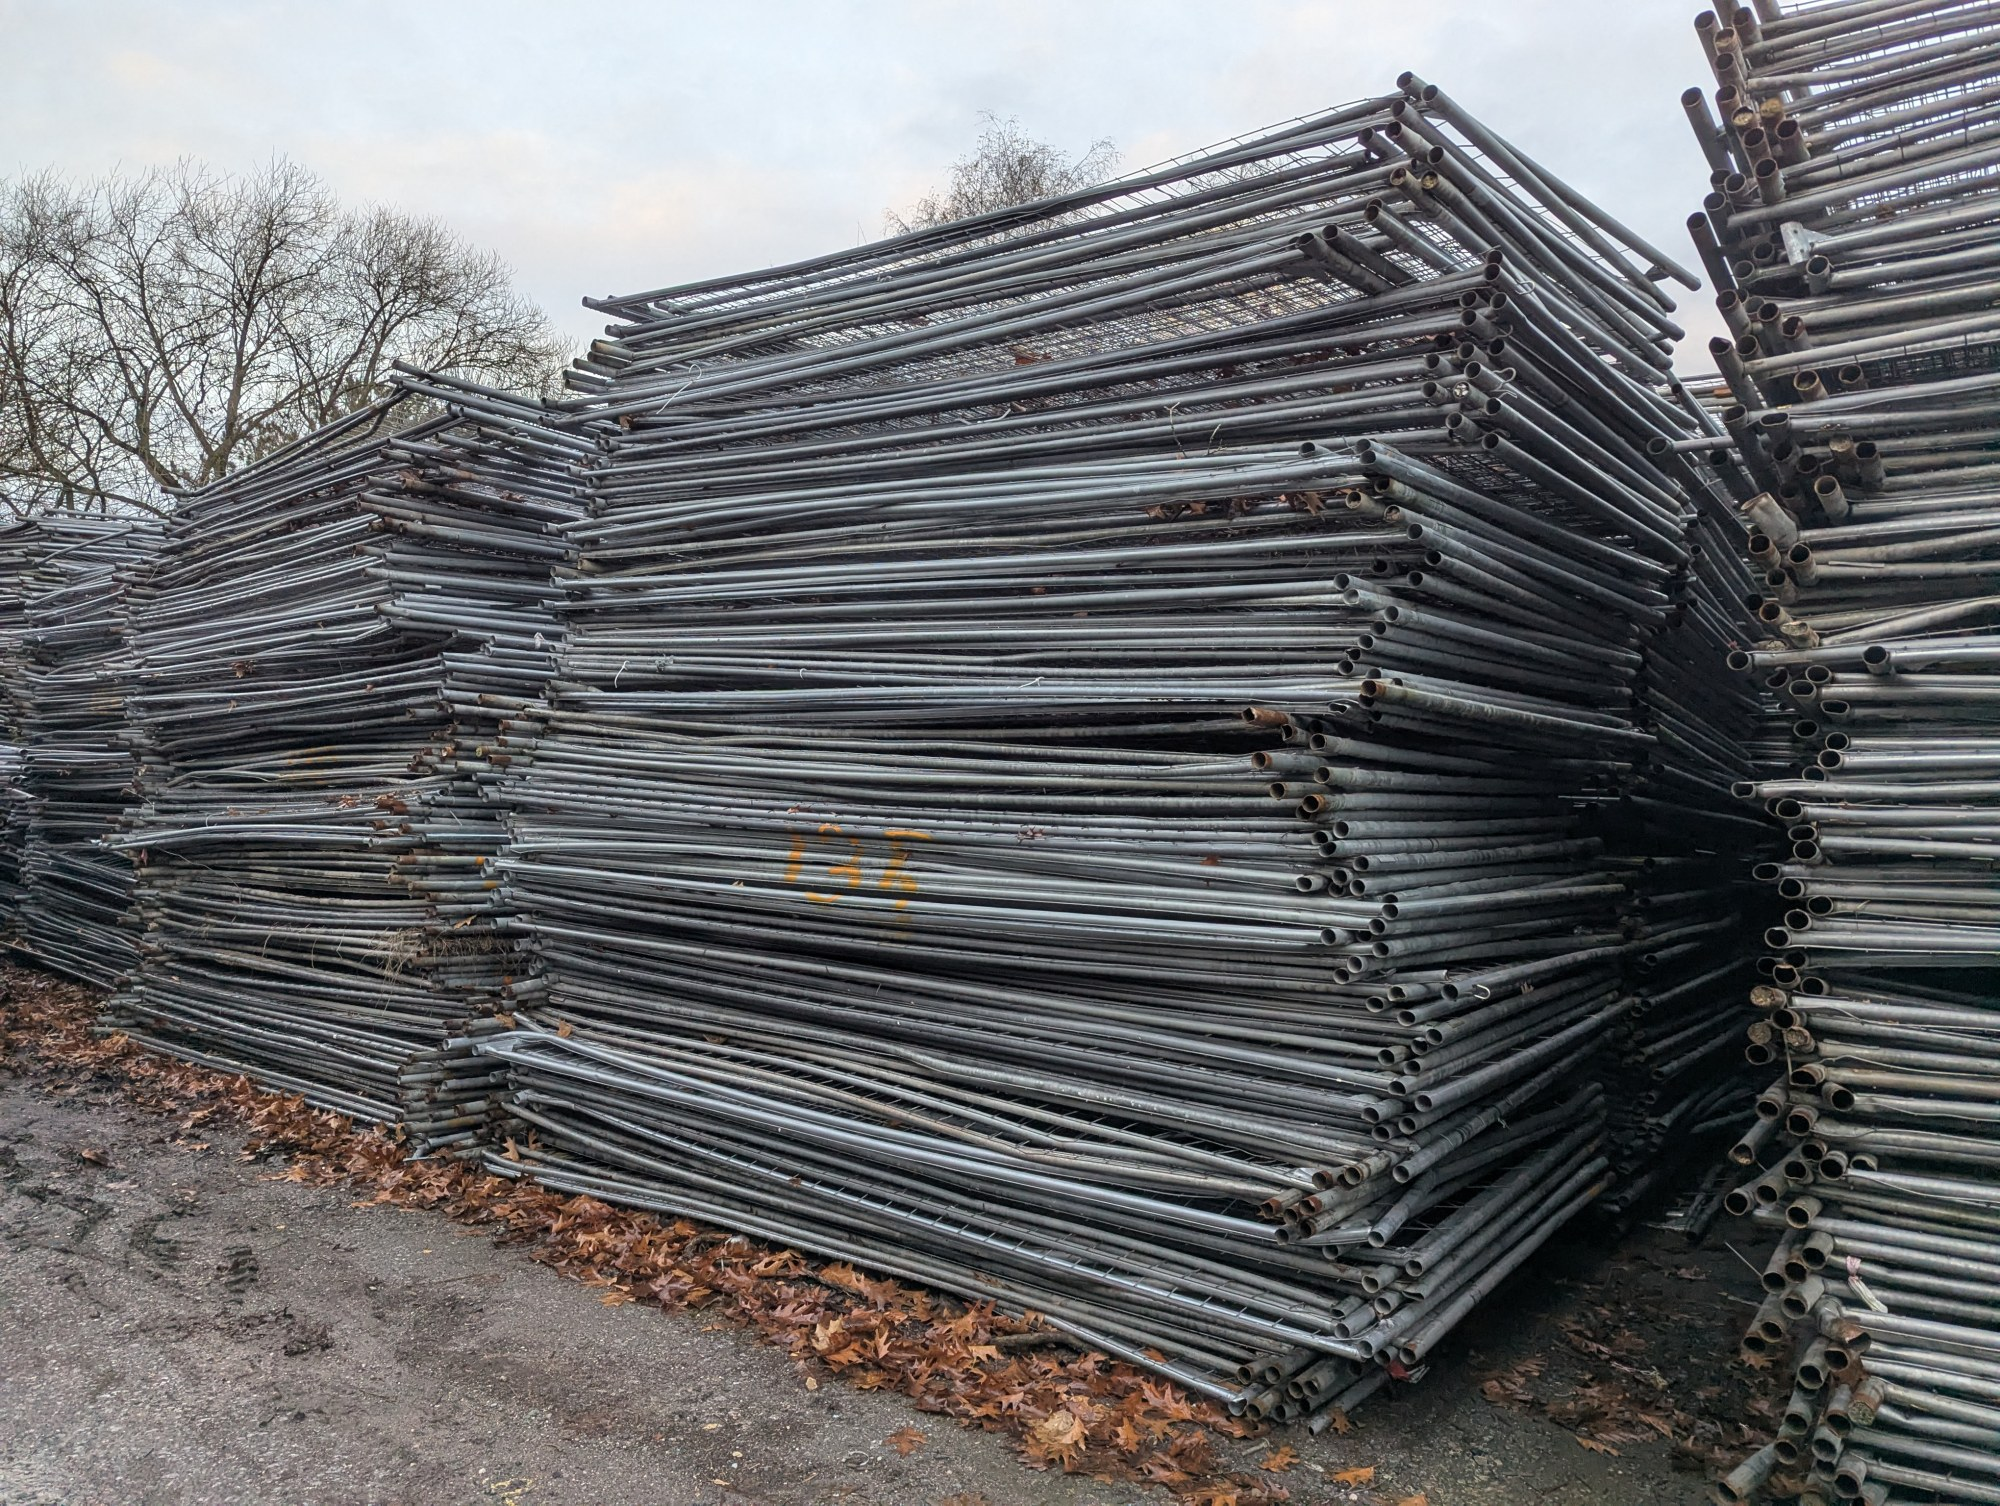
\includegraphics[width=0.52\textwidth]{abbildungen/real_stapel.jpg}
  \caption[Reale Stapelaufnahme]{Reale Aufnahme eines Stapels mobiler
  Bauzaunfelder. Zu detektieren ist die Stirnfläche der Rahmenrohre. Erkennbar
  sind die drei zentralen Schwierigkeiten: geringe Objektgröße, hohe
  Objektdichte und wechselseitige Verdeckung durch quer liegende Rohrschäfte.}
  \label{abb:realstapel}
\end{figure}

Aus Sicht der Bildverarbeitung ist das ein unangenehmer Spezialfall. Die Objekte
sind klein (gemessen 12--36\px{} Durchmesser im Original), dicht gepackt (im
Median rund ein Objektdurchmesser Abstand zum nächsten Nachbarn), untereinander
nahezu identisch und wechselseitig verdeckt. Erschwerend kommt hinzu, dass eine
Zählaufgabe jeden einzelnen Detektionsfehler unmittelbar in das Endergebnis
überträgt: Für eine exakte Zählung von 200 Objekten wäre eine Trefferquote von
über 99,5\,\% nötig.

Der eigentliche Engpass ist jedoch die Datenlage. COCO-vortrainierte Gewichte
enthalten keine Klasse \enquote{Bauzaunprofil}, und die Handannotation von
50--100 kleinen Boxen pro Bild über hunderte Bilder ist im Rahmen einer
Abschlussarbeit nicht leistbar. Zur Verfügung stehen neun aus Realbildern
ausgeschnittene Rohrprofile, sieben Hintergrundaufnahmen und zwei vollständig
annotierte Realbilder.

\section{Zielsetzung und Beitrag}

Der hier verfolgte Ansatz macht aus dieser Not das methodische Zentrum der
Arbeit: Trainiert wird \emph{ausschließlich} auf synthetischen Bildern, die aus
den neun Objektausschnitten und den sieben Hintergründen erzeugt werden;
Validierung und Test erfolgen auf den echten Aufnahmen. Damit ist die
Augmentierungspipeline nicht mehr eine Menge von Zusatztransformationen auf einem
vorhandenen Datensatz, sondern sie \emph{ist} der Datensatz: Sie definiert die
gesamte Trainingsverteilung.

Daraus ergibt sich die Gliederung der Arbeit, und es lohnt, die Rangfolge
ausdrücklich zu benennen. Ziel ist das \textbf{maschinelle Zählen} gestapelter
Bauzaunfelder. Der Schwerpunkt auf der Synthese-Pipeline ist diesem Ziel
\emph{nachgeordnet} und durch die Datenlage erzwungen: Ohne annotierte Realbilder
gibt es keinen Trainingsdatensatz, den man augmentieren könnte -- er muss erst
entstehen. Die untersuchten Architekturvarianten sind ein \emph{zweiter} Hebel
auf dieselbe Größe; sie stehen nicht in Konkurrenz zur Pipeline, sondern greifen
an derselben Ursache an, nämlich der geringen Objektgröße relativ zur
Gitterauflösung des Detektors. Entscheidungsmaß ist in beiden Fällen der
\textbf{Zählfehler} und nicht die mittlere Präzision -- eine Unterscheidung, die
sich in Abschnitt~\ref{sec:p2zaehlung} als folgenreich erweist.

Die Arbeit verfolgt drei Ziele. Erstens die \textbf{theoretische Einordnung der
Datenaugmentierung} (Kapitel~\ref{kap:augtheorie}): Was leistet Augmentierung
formal, welche Verfahrensklassen gibt es, welche Besonderheiten gelten bei der
Objektdetektion? Zweitens die \textbf{vollständige Dokumentation und Begründung
der konkreten Pipeline} (Kapitel~\ref{kap:pipeline} und
\ref{kap:trainingszeit}): Für jede Transformation werden Parameterbereich,
gemessener Ist-Anteil im erzeugten Datensatz und Begründung angegeben. Die
Begründung stützt sich dabei auf genau drei zulässige Quellen -- eine Messung an
den Realdaten, eine physikalische Randbedingung des Aufnahmegegenstands oder ein
in der Literatur belegtes Argument; wo keine dieser Quellen vorliegt, wird der
Wert ausdrücklich als Annahme gekennzeichnet. Drittens die
\textbf{experimentelle Bewertung} (Kapitel~\ref{kap:auswertung}) anhand von drei
Experimenten: Inferenzauflösung, Verdeckungsanteil in den Trainingsdaten und
Nutzen eines zusätzlichen hochauflösenden Detektionskopfes.

Der Beitrag liegt weniger in einer neuen Methode als in der Konsequenz, mit der
die Begründungspflicht durchgehalten wird. Copy-Paste-Synthese ist ein
etabliertes Verfahren \parencite{dwibedi2017,dvornik2018,ghiasi2021}; die Frage,
welche ihrer Bestandteile in einem konkreten industriellen Anwendungsfall tragen
und welche nicht, wird in der Literatur dagegen selten so kleinteilig
beantwortet.

\section{Aufbau}

Kapitel~\ref{kap:theorie} stellt die Grundlagen von Convolutional Neural Networks
und der YOLO26-Architektur bereit, Kapitel~\ref{kap:augtheorie} behandelt die
Datenaugmentierung allgemein und leitet sechs Anforderungen an die Pipeline ab.
Kapitel~\ref{kap:daten} vermisst das Quellmaterial -- diese Messungen sind die
Belegbasis aller Parameterentscheidungen. Kapitel~\ref{kap:pipeline} beschreibt
die Synthese-Pipeline, Kapitel~\ref{kap:trainingszeit} den Trainingsaufbau,
Kapitel~\ref{kap:auswertung} die Ergebnisse und Kapitel~\ref{kap:diskussion}
deren Tragfähigkeit und Grenzen; der Anhang nennt die Aufrufe der acht
Verarbeitungsstufen und enthält die vollständigen Parametertabellen.
